\IEEEraisesectionheading{\section{Introduction \label{sec-intro}}}

\IEEEPARstart{I}{n} recent years, recommender systems, which help users discover items of interest from a large resource collection, have been playing an increasingly important role in various online services~\cite{dias2008value,koren2015advances}.
Traditional recommendation methods (\eg matrix factorization) mainly aim to learn an effective prediction function for characterizing user-item interaction records (\eg user-item rating matrix). With the rapid development of web services, various kinds of auxiliary data (\aka side information) become available in recommender systems. Although auxiliary data is likely to contain useful information for recommendation~\cite{schafer2007collaborative},
it is difficult to model and utilize these heterogeneous and complex information in recommender systems.
Furthermore, it is more challenging to develop a relatively general approach to model these varying data in different systems or platforms.

As a promising direction, heterogeneous information network (HIN), consisting of multiple types of nodes and links, has been proposed as a powerful information modeling method~\cite{sun2011pathsim,shi2017survey,shi2017heterogeneous}.
 Due to its flexility in modeling data heterogeneity,
 HIN has been adopted in recommender systems to characterize rich auxiliary data.
In Fig.~\ref{fig_framework}(a), we present an example for movie recommendation characterized by HINs.
We can see that the HIN contains multiple types of entities connected by different types of relations.
Under the HIN based representation, the recommendation problem can be considered as a similarity search task over the HIN~\cite{sun2011pathsim}.
Such a recommendation setting is called as \emph{HIN based recommendation}~\cite{yu2013collaborative}.
HIN based recommendation has received much attention in the literature~\cite{feng2012incorporating,yu2013collaborative,yu2014personalized,shi2015semantic,shi2016integrating,zheng2017recommendation}.
 The basic idea of most existing HIN based recommendation methods is to leverage path based semantic relatedness between users and items over HINs, \eg meta-path based similarities,
 for recommendation.

\begin{figure*}[t]
\centering
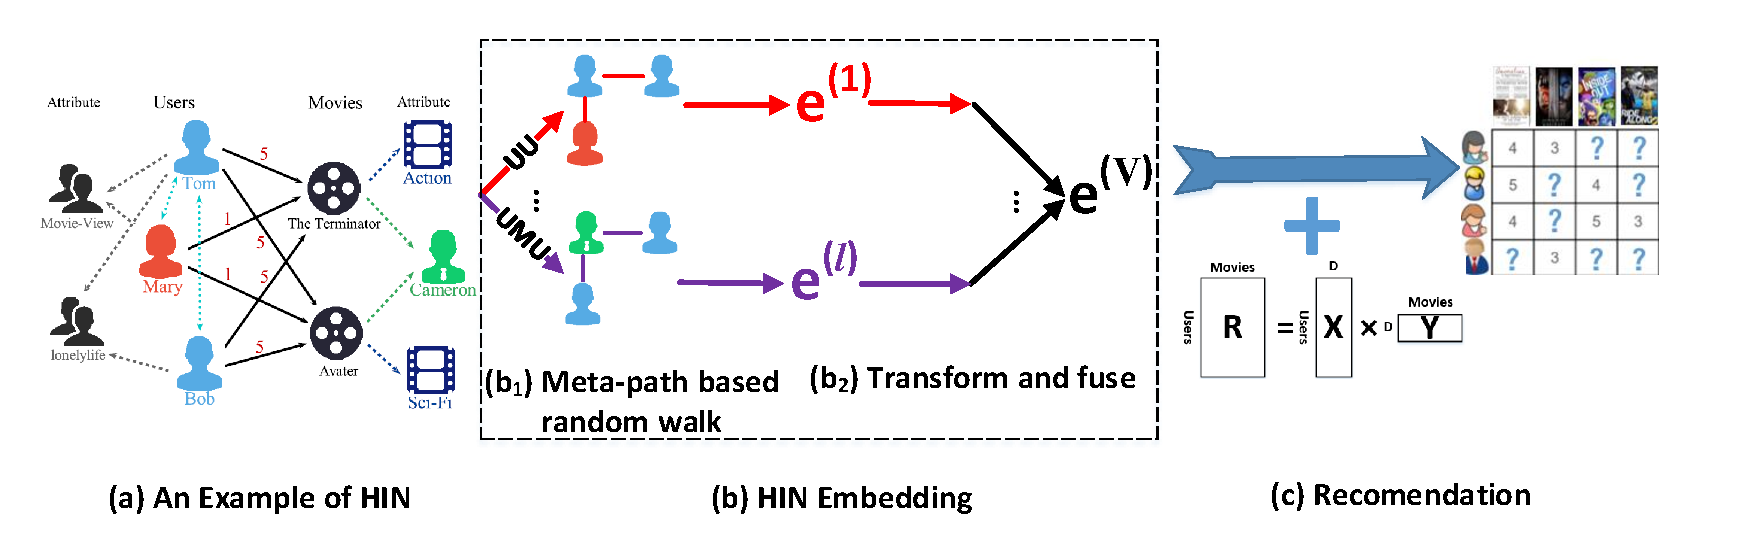
\includegraphics[width=15cm]{image/framework.pdf}
\caption{\label{fig_framework}The schematic illustration of the proposed HERec approach.}
\end{figure*}

Although HIN based methods have achieved performance improvement to some extent,
there are two major problems for these methods using meta-path based similarities.
First, meta-path based similarities rely on explicit path reachability,
and may not be reliable to be used for recommendation when
path connections are sparse or noisy.
It is likely that some links in HINs are accidentally formed which do not convey meaningful semantics.
Second, meta-path based similarities mainly characterize semantic relations defined over HINs, and may not be directly applicable to
recommender systems.
It is likely that the derived path based similarities have no explicit impact on the recommendation performance in some cases.
Existing methods mainly learn a linear weighting mechanism to combine the path based similarities~\cite{shi2016integrating} or latent factors~\cite{yu2013collaborative}, which cannot learn the complicated mapping mechanism of HIN information for recommendation.
The two problems essentially reflect two fundamental issues for HIN based recommendation, namely effective information extraction and exploitation based on HINs for recommendation.
%The focus of this paper is to study how to address these two issues and improve HIN-based recommendation.

For the first issue, it is challenging to develop a way to effectively extract and represent useful information for HINs due to data heterogeneity.
Unlike previous studies using meta-path based similarities~\cite{sun2011pathsim,yu2013collaborative}, our idea is to
learn effective heterogeneous network representations for summarizing important structural characteristics and properties of HINs.
Following \cite{perozzi2014deepwalk,grover2016node2vec}, we characterize nodes from HINs with low-dimensional vectors, \ie embeddings.
Instead of relying on explicit path connection, we would like to encode useful information from HINs with latent vectors.
Compared with meta-path based similarity, the learned embeddings are in a more compact form that is easy to use and integrate.
Also, the network embedding approach itself is more resistant to sparse and noisy data.
However, most existing network embedding methods focus on homogeneous networks only consisting of a single type of nodes and links, and cannot directly deal with heterogeneous networks consisting of multiple types of nodes and links. Hence, we propose a new heterogeneous network embedding method.
Considering heterogeneous characteristics and rich semantics reflected by meta-paths, the proposed method first uses a
random walk strategy guided by meta-paths to generate node sequences. For each meta-path, we learn a unique embedding representation for a node by maximizing its co-occurrence probability with neighboring nodes in the sequences sampled according to the given meta-path. We fuse the multiple embeddings \emph{w.r.t.} different meta-paths as the output of HIN embedding.

After obtaining the embeddings from HINs, we study how to integrate and utilize such information in recommender systems.
We don't assume the learned embeddings are naturally applicable in recommender systems. Instead, we propose and explore three fusion functions to integrate multiple embeddings of a node into a single representation for recommendation, including simple linear fusion, personalized linear fusion and non-linear fusion.
These fusion functions provide flexible ways to transform HIN embeddings into useful information for recommendation.
Specially, we emphasize that personalization and non-linearity are two key points to consider for information transformation in our setting.
Finally, we extend the classic matrix factorization framework by incorporating the fused HIN embeddings.
The prediction model and the fusion function are jointly optimized for the rating prediction task.

By integrating the above two parts together, this work presents a novel HIN embedding based recommendation approach, called \emph{HERec} for short.
HERec first extracts useful HIN based information using the proposed HIN embedding method,
and then utilizes the extracted information for recommendation using the extended matrix factorization model.
We present the overall illustration for the proposed approach in Fig.~\ref{fig_framework}.
Extensive experiments on three real-world datasets demonstrate the effectiveness of the proposed approach. We also  verify the ability of HERec to alleviate cold-start problem and examine the impact of meta-paths on performance. The key contributions of this paper can be summarized as follows:


\textbullet ~We propose a heterogeneous network embedding method guided by meta-paths to uncover the semantic and structural information of heterogeneous information networks. Moreover, we propose a general embedding fusion approach to integerate different
embeddings based on different meta-paths into a single representation.

\textbullet ~We propose a novel heterogeneous information network embedding for recommendation model, called HERec for short. HERec can effectively integrate various kinds of embedding information in HIN to enhance the recommendation performance. In addition, we design a set of three flexible fusion functions to effectively transform HIN embeddings into useful information for recommendation.

\textbullet ~Extensive experiments on three real-world datasets demonstrate the effectiveness of the proposed model. Moreover, we show the capability of the proposed model for the cold-start prediction problem, and reveal that the transformed embedding information from HINs can improve the recommendation performance.

The remainder of this paper is organized as follows. Section~\ref{sec-rel} introduces the related works. Section~\ref{sec-def} describes notations used in the paper and presents some preliminary knowledge. Then, We propose the heterogeneous network embedding method and the HERec model in Section~\ref{sec-model}. Experiments and detailed analysis are reported in Section~\ref{sec-exp}. Finally, we conclude the paper in Section~\ref{sec-con}.

\begin{figure*}[t]
\centering
\subfigure[Douban Movie]{
\begin{minipage}[b]{0.3\textwidth}
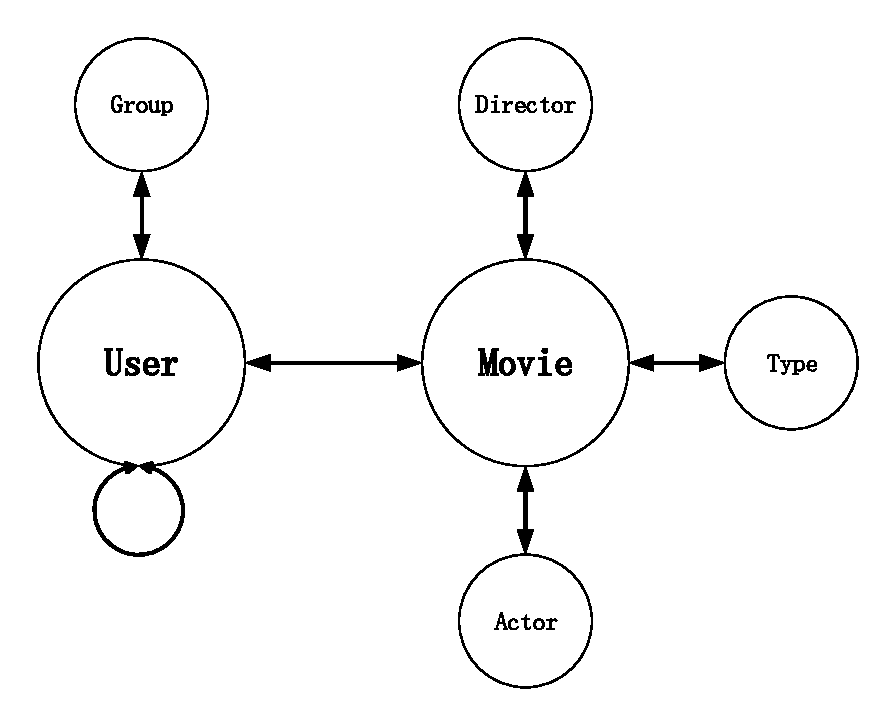
\includegraphics[width=1\textwidth]{image/doubanmovie.pdf}
\end{minipage}
}
\subfigure[Douban Book]{
\begin{minipage}[b]{0.3\textwidth}
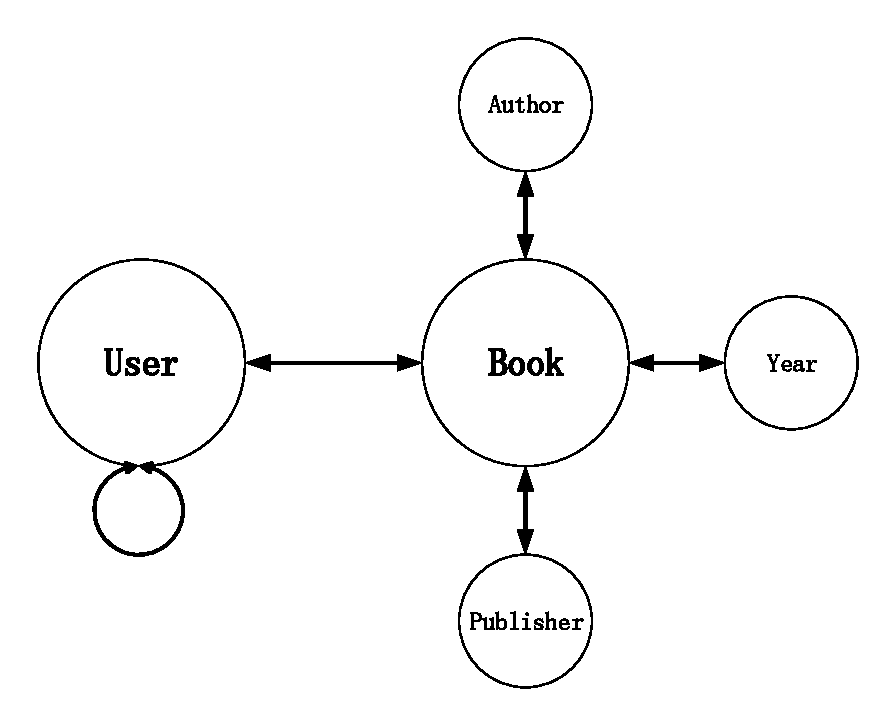
\includegraphics[width=1\textwidth]{image/doubanbook.pdf}
\end{minipage}
}
\subfigure[Yelp]{
\begin{minipage}[b]{0.3\textwidth}
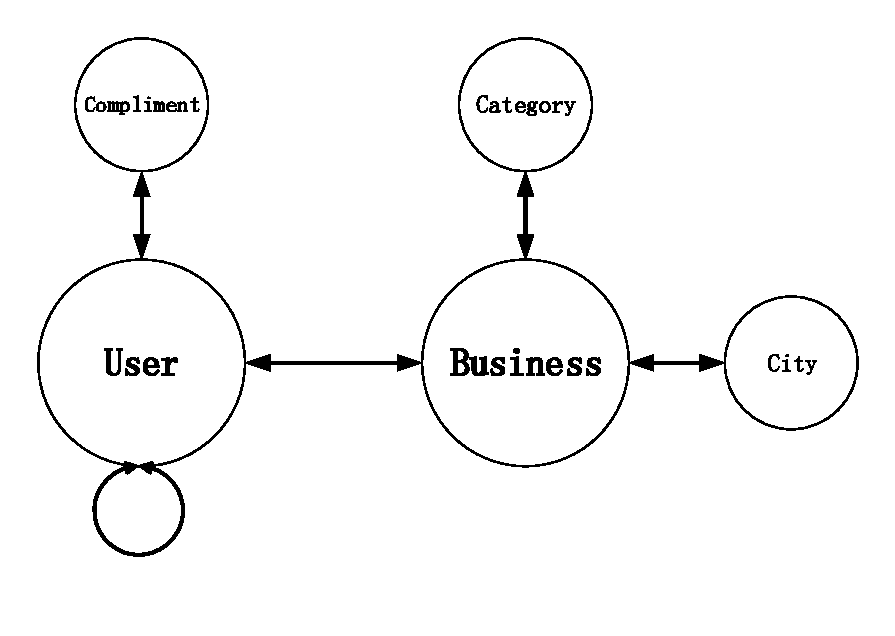
\includegraphics[width=1\textwidth]{image/yelp.pdf}
\end{minipage}
}
\caption{\label{fig_schema}Network schemas of heterogeneous information networks for the used three datasets.
In our task, users and items are our major focus, denoted by large-sized circles, while the other attributes are denoted by small-sized circles. }

\end{figure*}

